% -*- latex -*-
%%%%%%%%%%%%%%%%%%%%%%%%%%%%%%%%%%%%%%%%%%%%%%%%%%%%%%%%%%%%%%%%
%%%%%%%%%%%%%%%%%%%%%%%%%%%%%%%%%%%%%%%%%%%%%%%%%%%%%%%%%%%%%%%%
%%%%
%%%% This text file is part of the source of 
%%%% `Parallel Computing'
%%%% by Victor Eijkhout, copyright 2012/3
%%%%
%%%%%%%%%%%%%%%%%%%%%%%%%%%%%%%%%%%%%%%%%%%%%%%%%%%%%%%%%%%%%%%%
%%%%%%%%%%%%%%%%%%%%%%%%%%%%%%%%%%%%%%%%%%%%%%%%%%%%%%%%%%%%%%%%

This section gives reference information and illustrative examples
of the use of MPI. While the code snippets given here should be enough,
full programs can be found in the repository for this book
\url{https://bitbucket.org/VictorEijkhout/parallel-computing-book}.

\Level 0 {Basics}

\Level 1 {MPI setup}
\commandreflabel{mpi-init}

If you use MPI commands in a program file, be sure to include
the proper header file, \indexterm{mpi.h} or \indexterm{mpif.h}.
\begin{verbatim}
#include "mpi.h" // for C
#include "mpif.h" ! for Fortran
\end{verbatim}
For \indexterm{Fortran90}, many MPI installations also have an MPI
module, so you can write
\begin{verbatim}
use mpi
\end{verbatim}
The internals of these files can be different between MPI
installations, so you can not compile one file against one \n{mpi.h}
file and another file, even with the same compiler on the same machine,
against a different MPI.

Every MPI program has to start with\indexmpi{MPI_Init}
\begin{verbatim}
MPI_Init(&argc,&argv);
\end{verbatim}
where \indextermtt{argc} and \indextermtt{argv} are the arguments
of a C language main program:
\begin{verbatim}
int main(int argc,char **argv) {
    ....
    return 0;
}
\end{verbatim}
The regular way to conclude an MPI program is through\indexmpi{MPI_Finalize}
\begin{verbatim}
MPI_Finalize();
\end{verbatim}
but an abnormal end to a run can be forced by\indexmpi{MPI_Abort}
\begin{verbatim}
MPI_Abort(comm,value);
\end{verbatim}
This aborts execution on all processes associated with the communicator,
but many implementations simply abort all processes. The \n{value} parameter
is returned to the environment.

The corresponding Fortran calls are
\begin{verbatim}
call MPI_Init(ierr)
// your code
call MPI_Finalize()
\end{verbatim}
Note that the \n{MPI_Init} call is one of the few that differs between C and Fortran:
the C~routine takes the commandline arguments, which Fortran lacks.

Any \indexterm{commandline argument} to the program can only be
guaranteed to be passed correctly to process zero. Here is a fragment
of code that shows use of commandline arguments.  The program
\n{examples/mpi/c/init.c} takes a single integer commandline argument.
If the user forgets to specify an argument of specifies~\n{-h}, a
usage message is printed and the program aborts, otherwise the
parameter is broadcast to all processes.  
%
\verbatimsnippet{usage}
%
For Fortran:
%
\verbatimsnippet{usage-f}

\Level 1 {MPI ranks and communicator sizes}
\commandreflabel{rank-size}

Every MPI process has its own local storage. So if you pretend that all these
small arrays are really together one big array, you need to know where each 
piece fits in the whole. For this you need to know at the very least
how many processes there are and what the rank of a process is.

The following example creates a distributed array that will contains
the values of a function at equidistant points in the interval~$[0,1]$.
The code implements this as follows:
\begin{enumerate}
\item each process has an array of 10 points,
\item so the distributed array has a length of 10 times the number of processes;
\item of this array, each process has 10 points, starting at 10 times
  the process id.
\item To fill in values in the local array, the process iterates only
  over its local points,
\item but it needs to calculate the global coordinate of those points.
\end{enumerate}
 
\verbatimsnippet{local}

\Level 1 {Send and receive buffers}

The data is specified as a number of elements in a buffer. The same
MPI routine can be used with data of different types, so the standard
indicates such buffers as \indexterm{choice}. The specification of
this differs per language:
\begin{itemize}
\item In C it is an address, so the clean way is to pass it as
  \verb+(void*)&myvar+.
\item Fortran compilers may complain about type mismatches. This can
  not be helped.
\end{itemize}

\Level 0 {Data types}

\Level 1 {Elementary types}
\commandreflabel{elementary}
\index{datatype!elementary|(}

C/C++:

\begin{tabular}{ll}
\n{MPI_CHAR}&only for text data, do not use for small integers\\
\n{MPI_UNSIGNED_CHAR}\\
\n{MPI_SIGNED_CHAR}\\
\n{MPI_SHORT}\\
\n{MPI_UNSIGNED_SHORT}\\
\n{MPI_INT}\\
\n{MPI_UNSIGNED}\\
\n{MPI_LONG}\\
\n{MPI_UNSIGNED_LONG}\\
\n{MPI_FLOAT}\\
\n{MPI_DOUBLE}\\
\n{MPI_LONG_DOUBLE}
\end{tabular}

There is some, but not complete, support for \indexterm{C99} types.

Fortran:

\begin{tabular}{ll}
\n{MPI_CHARACTER}&Character(Len=1)\\
\n{MPI_LOGICAL}\\
\n{MPI_INTEGER}\\
\n{MPI_REAL}\\
\n{MPI_DOUBLE_PRECISION}\\
\n{MPI_COMPLEX}\\
\n{MPI_DOUBLE_COMPLEX}&Complex(Kind=Kind(0.d0))\\
\end{tabular}

Addresses have type \indexmpishow{MPI_Aint} or \n{INTEGER
(KIND=MPI_ADDRESS_KIND)} in Fortran. The start of the address range is
given in \indexmpishow{MPI_BOTTOM}.

\index{datatype!elementary|)}

\Level 1 {Derived datatypes}
\commandreflabel{derived-types}
\index{datatype!derived|(}

The space taken by a derived type is not immediately obvious from its
definition since padding maybe applied. The actual size can be
retrieved with \indexmpishow{MPI_Type_extent}:
\begin{verbatim}
int MPI_Type_extent(MPI_Datatype datatype, MPI_Aint *extent)
\end{verbatim}
See the example in section~\ref{ref:data:struct}

\Level 2 {Type create and release calls}
\commandreflabel{data-commit}

A derived type needs to be committed with \indexmpishow{MPI_Type_commit}:
\begin{verbatim}
int MPI_Type_commit (MPI_datatype *datatype)
\end{verbatim}
The commit call is typically used to find an efficient `flat' representation
of recursively defined datatypes.

When you no longer need the derived type, its space can be released with
\indexmpishow{MPI_Type_free}:
\begin{verbatim}
int MPI_Type_free (MPI_datatype *datatype)
\end{verbatim}
After the type free call
\begin{itemize}
\item The definition of the datatype identifier will be changed to
  \indexmpishow{MPI_DATATYPE_NULL}.
\item Any communication using this data type, that was already
  started, will be completed succesfully.
\item Datatypes that are defined in terms of this data type will still
  be usable.
\end{itemize}

\Level 2 {Contiguous type}
\commandreflabel{data:contiguous}

A contiguous datatype, created with a call to \indexmpishow{MPI_Type_contiguous},
\begin{verbatim}
int MPI_Type_contiguous(
  int count, MPI_Datatype old_type, MPI_Datatype *new_type_p)
\end{verbatim}
consists of a number of elements of a datatype, contiguous in memory.
Sending one element of a contiguous type is fully equivalent to sending
a number of elements of the constituent type.
\verbatimsnippet{contiguous}

\Level 2 {Vector type}
\commandreflabel{data:vector}

The \indexmpishow{MPI_Type_vector} type can be used to create a type
of regularly spaced blocks of data. All block lengths need to be the same,
and the vector type is built out of a single constituent type.
\begin{verbatim}
int MPI_Type_vector(
  int count, int blocklength, int stride,
  MPI_Datatype old_type, MPI_Datatype *newtype_p
);
\end{verbatim}

In this example a vector type is created only on the sender, in order to send
a strided subset of an array; the receiver receives the data as a contiguous block.
\verbatimsnippet{vector}

\Level 2 {Indexed data}
\commandreflabel{data:indexed}

The indexed datatype is similar to the vector type, in the sense that it consists
of a series of blocks of items, all of the same type. However, where the
vector type was described by a single stride and blocklength,
with \indexmpishow{MPI_Type_indexed}
you can specify the location and length of each block.
\begin{verbatim}
int MPI_Type_indexed(
  int count, int blocklens[], int indices[],
  MPI_Datatype old_type, MPI_Datatype *newtype);
\end{verbatim}
The following example picks items that are on prime number-indexed
locations.
\verbatimsnippet{indexed}

You can also \indexmpishow{MPI_Type_create_hindexed} which describes blocks
of a single old type, but with indix locations in bytes, rather than
in multiples of the old type.
\begin{verbatim}
int MPI_Type_create_hindexed
 (int count, int blocklens[], MPI_Aint indices[],
  MPI_Datatype old_type,MPI_Datatype *newtype)
\end{verbatim}
You can use this to pick all occurrences of a single component out of
an array of structures. However, you need to be very careful with the
index calculation. Use pointer arithmetic, as in the example in
section~\ref{ref:data:struct}.  Another use of this function is in
sending an \n{stl<vector>}\index{C++!standard library!vector}, that
is, a vector object from the \indextermbus{C++}{standard library}, if
the component type is a pointer. No further explanation here.

\Level 2 {Structure data}
\commandreflabel{data:struct}

The \indexmpishow{MPI_Type_create_struct} routine creates
a type consisting of blocks of multiple datatypes,
much like \n{MPI_Type_indexed} makes
an array of blocks of a single type.
\begin{verbatim}
int MPI_Type_create_struct(
  int count, int blocklengths[], MPI_Aint displacements[],
  MPI_Datatype types[], MPI_Datatype *newtype);
\end{verbatim}
\begin{description}
\item[\texttt{count}] The number of blocks in this
  datatype. The \n{blocklengths}, \n{displacements}, \n{types}
  arguments have to be at least of this length.
\item[\texttt{blocklengths}] array containing the lengths of the blocks of each datatype.
\item[\texttt{displacements}] array describing the relative location
  of the blocks of each datatype.
\item[\texttt{types}] array containing the datatypes; each block in
  the new type is of a single datatype; there can be multiple
  blocks consisting of the same type.
\end{description}
In this example, unlike the previous ones, both sender and receiver
create the structure type. With structures it is no longer possible to
send as a derived type and receive as a array of a simple type.
(It would be possible to send as one structure type and receive as another, 
as long as they have the same \indextermbus{datatype}{signature}.)
\verbatimsnippet{structure}
Note the \n{displacement} calculations in this example,
which involve some not so elegant pointer arithmetic.
It would have been incorrect to write
\begin{verbatim}
displacement[0] = 0;
displacement[1] = displacement[0] + sizeof(char);
\end{verbatim}
since you do not know the way the \indexterm{compiler} lays out the
structure in memory\footnote{Homework question: what does the language
  standard say about this?}.
The space that MPI takes for a structure type can be queried 
with \indexmpishow{MPI_Type_extent}.

(There is a deprecated function \indexmpishow{MPI_Type_struct} with the same
functionality.)

\index{datatype!derived|)}

\Level 1 {Packed data}
\commandreflabel{pack}

With \indexmpishow{MPI_PACK} data elements can be added 
to a buffer one at a time. The \n{position} parameter is updated
each time by the packing routine.
\begin{verbatim}
int MPI_Pack(
  void *inbuf, int incount, MPI_Datatype datatype,
  void *outbuf, int outcount, int *position,
  MPI_Comm comm);
\end{verbatim}

Conversely, \indexmpishow{MPI_UNPACK} retrieves one element
from the buffer at a time. You need to specify the MPI datatype.
\begin{verbatim}
int MPI_Unpack(
  void *inbuf, int insize, int *position,
  void *outbuf, int outcount, MPI_Datatype datatype,
  MPI_Comm comm);
\end{verbatim}

A packed buffer is sent of received with a datatype of
\indexmpishow{MPI_PACKED}. The sending routine uses the \n{position}
parameter to specify how much data is sent, but the receiving routine
does not know this value a~priori, so has to specify an upper bound.

\verbatimsnippet{packunpack}

\Level 0 {Blocking communication}
\commandreflabel{blocking}

The basic send command is \indexmpishow{MPI_Send}:
\begin{verbatim}
int MPI_Send(void *buf, 
  int count, MPI_Datatype datatype, int dest, int tag,
  MPI_Comm comm)
\end{verbatim}
\url{http://www.mcs.anl.gov/research/projects/mpi/www/www3/MPI_Send.html}
This routine may not blocking for small messages; to force blocking
behaviour use \n{MPI_Ssend} with the same argument list.
\url{http://www.mcs.anl.gov/research/projects/mpi/www/www3/MPI_Ssend.html}

The basic blocking receive command is \indexmpishow{MPI_Recv}:
\begin{verbatim}
int MPI_Recv(void *buf, 
  int count, MPI_Datatype datatype, int source, int tag,
  MPI_Comm comm, MPI_Status *status)
\end{verbatim}
\url{http://www.mcs.anl.gov/research/projects/mpi/www/www3/MPI_Recv.html}
The \n{count} argument indicates the maximum length of a message; the
actual length of the received message can be determined 
from the status object. See section~\ref{ref:mpi-source}
for more about the status object.

The following code is guaranteed to block, since a \n{MPI_Recv}
always blocks:
\verbatimsnippet{recvblock}
On the other hand, if we put the send call before the receive,
code may not block for small messages
that fall under the \indexterm{eager limit}. In this example we send
gradually larger messages. From the screen output you can see what
the largest message was that fell under the eager limit; after that the code
hangs because of a deadlock.
%
\verbatimsnippet{sendblock}
%
\verbatimsnippet{sendblock-f}
%
If you want a code to behave the same for all message sizes,
you force the send call to be blocking by using \n{MPI_Ssend}:
\verbatimsnippet{ssendblock}

\Level 1 {Receive status}
\commandreflabel{mpi-source}

Any time you receive data, there can be an \indexmpishow{MPI_Status}
object describing the data that was received. This can be necessary if
you use \indexmpishow{MPI_ANY_SOURCE} or \indexmpishow{MPI_ANY_TAG} in
the description of the receive message. If you are not interested in
the status information, you can use the values
\indexmpishow{MPI_STATUS_IGNORE} or (for \indexmpishow{MPI_Waitall},
\indexmpishow{MPI_Waitany}) \indexmpishow{MPI_STATUSES_IGNORE}.

A receive call has a \n{count} parameter, but this describes the length
of the buffer, not the amount of data expected. That quantity
can be retrieved with \indexmpishow{MPI_Get_count}.
\begin{verbatim}
// C:
int MPI_Get_count(MPI_Status *status,MPI_Datatype datatype,
    int *count)
! Fortran:
MPI_Get_count(INTEGER status(MPI_STATUS_SIZE),INTEGER datatype,
    INTEGER count,INTEGER ierror)
\end{verbatim}

The status object is returned when the message is received. Thus, with
\n{MPI_Recv} it is returned explicitly,
but with \n{MPI_Irecv} it is returned from the \n{MPI_Wait...} call.
\begin{fortrannote}
  In Fortran the \n{MPI_Status} object needs to be explicitly created:
\begin{verbatim}
integer status(MPI_STATUS_SIZE)
\end{verbatim}
\end{fortrannote}

In section~\ref{sec:mpi-source} we mentioned the master-worker model
as one opportunity for inspecting the \indexmpishow{MPI_SOURCE} field
of the \indexmpishow{MPI_Status} object. Here is a small example: 
the tasks perform a variable amount of work (modeled here by a random wait)
before sending a message to the master. The master waits for any source,
and inspects the status field to report where the message comes from.

\verbatimsnippet{anysource}

\Level 0 {Deadlock-free blocking messages}
\commandreflabel{send-recv}

If messsages are send roughly in pairs, the 
\indexmpishow{MPI_Sendrecv} call is an easy way to prevent deadlock.
Here you specify both the target of a send and the source of a receive,
which can be same in case of a pairwise exchange of data,
but they need not be the same. To swap equal-sized buffers you
can use \indexmpishow{MPI_Sendrecv_replace}.
\begin{verbatim}
int MPI_Sendrecv(
  void *sendbuf, int sendcount, MPI_Datatype sendtype, 
        int dest, int sendtag,
  void *recvbuf, int recvcount, MPI_Datatype recvtype, 
        int source, int recvtag,
  MPI_Comm comm, MPI_Status *status)
int MPI_Sendrecv_replace(
  void *buf, int count, MPI_Datatype datatype, 
        int dest, int sendtag,
        int source, int recvtag,
  MPI_Comm comm, MPI_Status *status)
\end{verbatim}

As an example we set up a ring of three processors: each process sends
to its right neighbour, and receives from its left neighbour.
\verbatimsnippet{sendrecvring}

\Level 0 {Non-blocking communication}
\commandreflabel{nonblocking}

The non-blocking routines have much the same parameter list as the 
blocking ones, with the addition of an \indexmpishow{MPI_Request} parameter.
The \n{MPI_Isend} routine does not have an \indexmpishow{MPI_Status} parameter,
which has moved to the `wait' routine.
\begin{verbatim}
int MPI_Isend(void *buf,
  int count, MPI_Datatype datatype, int dest, int tag,
  MPI_Comm comm, MPI_Request *request)
\end{verbatim}
\url{http://www.mcs.anl.gov/research/projects/mpi/www/www3/MPI_Isend.html}
\begin{verbatim}
int MPI_Irecv(void *buf,
  int count, MPI_Datatype datatype, int source, int tag,
  MPI_Comm comm, MPI_Request *request)
\end{verbatim}
\url{http://www.mcs.anl.gov/research/projects/mpi/www/www3/MPI_Irecv.html}

\begin{fortrannote}
  The request parameter is an integer.
\end{fortrannote}

There are various `wait' routines. Since you will often do at least
one send and one receive, this routine is useful:
\begin{verbatim}
int MPI_Waitall(int count, MPI_Request array_of_requests[], 
  MPI_Status array_of_statuses[])
\end{verbatim}
\url{http://www.mcs.anl.gov/research/projects/mpi/www/www3/MPI_Waitall.html}

Here is a simple code that does a non-blocking exchange between two processors:
\verbatimsnippet{irecvnonblock}

It is possible to omit the status array by specifying \indexmpishow{MPI_STATUSES_IGNORE}.
Other routines are \n{MPI_Wait} for a single request, and
\n{MPI_Waitsome}, \n{MPI_Waitany}.

The above fragment is unrealistically simple. In a more general scenario we
have to manage send and receive buffers: we need as many buffers as there are
simultaneous non-blocking sends and receives.
\verbatimsnippet{irecvloop}

Instead of waiting for all messages, we can wait for any message to come
with \indexmpishow{MPI_Waitany}, and process the receive data as it comes in.
\verbatimsnippet{waitforany}
Note the \indexmpishow{MPI_STATUS_IGNORE} parameter: we know everything
about the incoming message, so we do not need to query a status object.
Contrast this with the example in section~\ref{ref:mpi-source}.

\begin{fortrannote}
  The \n{index} parameter is the index in the array of requests,
  so it uses \emph{1-based indexing}\index{fortran!1-based indexing}.
\end{fortrannote}
\verbatimsnippet{waitforany-f}

\Level 1 {Persistent communication}
\commandreflabel{persistent}
\index{communication!persistent|(}

The calls \indexmpishow{MPI_Send_init} and \indexmpishow{MPI_Recv_init}
for creating a persistent communication have the same syntax as 
those for non-blocking sends and receives. The difference is that they do not start
an actual communication, they only create the request object.
\begin{verbatim}
int MPI_Send_init(
  void* buf, int count, MPI_Datatype datatype, 
  int dest, int tag, MPI_Comm comm, MPI_Request *request) 
int MPI_Recv_init(
  void* buf, int count, MPI_Datatype datatype, 
  int source, int tag, MPI_Comm comm, 
  MPI_Request *request)
\end{verbatim}

Given these request object, a communication (both send and receive) is then started
with \indexmpishow{MPI_Start} for a single request or \indexmpishow{MPI_Start_all} for 
multiple requests, given in an array.
\begin{verbatim}
int MPI_Start(MPI_Request *request)
int MPI_Startall(int count, MPI_Request *array_of_requests) 
\end{verbatim}
These are equivalent to starting an \n{Isend} or \n{Isend}; correspondingly, 
it is necessary to issue an \n{MPI_Wait...} call (section~\ref{ref:nonblocking})
to determine their completion.

After a request object has been used, possibly multiple times, it can be freed; see~\ref{ref:mpirequest}.

In the following example a ping-pong is implemented with persistent communication.
\verbatimsnippet{persist}

As with ordinary send commands, there are the variants
\indexmpishow{MPI_Bsend_init},
\indexmpishow{MPI_Ssend_init},
\indexmpishow{MPI_Rsend_init}.

\index{communication!persistent|)}

\Level 1 {About \texttt{MPI\_Request}}
\label{ref:mpirequest}

An \indexmpidef{MPI_Request} object is not actually an object,
unlike \n{MPI_Status}. Instead it is an (opaque) pointer.
This meeans that when you call, for instance, \n{MPI_Irecv},
MPI will allocate an actual request object, and return its
address in the \n{MPI_Request} variable.

Correspondingly, calls to \indexmpishow{MPI_Wait...} or \indexmpishow{MPI_Test}
free this object.
If your application is such that you do not use `wait' call, you can free the
request object explicitly
with \indexmpishow{MPI_Request_free}.
\begin{verbatim}
int MPI_Request_free(MPI_Request *request)
\end{verbatim}

You can inspect the status of a request without freeing the request object
with \indexmpishow{MPI_Request_get_status}:
\begin{verbatim}
int MPI_Request_get_status(
  MPI_Request request,
  int *flag,
  MPI_Status *status
);
\end{verbatim}

\Level 0 {One-sided communication}
\commandreflabel{one-sided}

\Level 1 {Windows and epochs}
\commandreflabel{windows}

C syntax for \indexmpishow{MPI_Win_create}
\begin{verbatim}
MPI_Win_create (void *base, MPI_Aint size, 
  int disp_unit, MPI_Info info, 
  MPI_Comm comm, MPI_Win *win)
\end{verbatim}
The data array must not be \n{PARAMETER} or \n{static const}.

The size parameter is measured in bytes. In~C this is easily done
with the \indextermtt{sizeof} operator;
for doing this calculation in Fortran, see section~\ref{sec:f-sizeof}.

The \indexmpishow{MPI_Info} parameter can be used to pass implementation-dependent 
information:
\begin{verbatim}
MPI_Info info;
MPI_Info_create(&info);
MPI_Info_set(info,"no_locks","true");
MPI_Win_create( ... info ... &win);
MPI_Info_free(&info);
\end{verbatim}
It is always valid to use \indexmpishow{MPI_INFO_NULL}.

\indexmpishow{MPI_Alloc_mem}
\begin{verbatim}
int MPI_Alloc_mem(MPI_Aint size, MPI_Info info, void *baseptr)
\end{verbatim}

\Level 1 {Remote memory access}
\commandreflabel{putget}

C interface to \indexmpi{MPI_Put}:
\begin{verbatim}
MPI_Put (
  void *origin_addr, int origin_count, MPI_Datatype origin_datatype,
  int target_rank,
  MPI_Aint target_disp, int target_count, MPI_Datatype target_datatype,
  MPI_Win window)
\end{verbatim}
Fortran interface
\begin{verbatim}
MPI_Put(origin_addr, origin_count, origin_datatype, target_rank,
    target_disp, target_count, target_datatype, win, ierror)

<type> :: origin_addr(*)
INTEGER(KIND=MPI_ADDRESS_KIND) :: target_disp
INTEGER :: origin_count, origin_datatype,
    target_rank, target_count, target_datatype,
    win, ierror
\end{verbatim}


The \indexmpishow{MPI_Get} call is very similar.
\begin{verbatim}
int MPI_Get(void *origin_addr, int origin_count, MPI_Datatype
            origin_datatype, int target_rank, MPI_Aint target_disp,
            int target_count, MPI_Datatype target_datatype, MPI_Win
            win)
\end{verbatim}

Here is a single put operation. Note that the window create and window fence calls
are collective, so they have to be performed on all processors
of the communicator that was used in the create call.
\verbatimsnippet{putblock}

Very similar, a get operation.
\verbatimsnippet{getblock}

A third one-sided routine
is \n{MPI_Accumulate} which does a reduction operation on the results
that are being put:\indexmpi{MPI_Accumulate}
\begin{verbatim}
MPI_Accumulate (
  void *origin_addr, int origin_count, MPI_Datatype origin_datatype, 
  int target_rank,
  MPI_Aint target_disp, int target_count, MPI_Datatype target_datatype,
  MPI_Op op,MPI_Win window)
\end{verbatim}

\Level 1 {Active target synchronization}
\commandreflabel{fence}

\indexmpi{MPI_Win_fence}
\begin{verbatim}
MPI_Win_fence (int assert, MPI_Win win)
\end{verbatim}

\Level 1 {Assertions}
\label{sec:mpi-assert}

The \n{MPI_Win_fence} call, as well \n{MPI_Win_start} and such, take an argument
through which assertions can be passed about the activity before, after, and during the epoch.
The value zero is always allowed, by you can make your program more efficient by specifying
one or more of the following:
\begin{itemize}
\item \indexmpishow{MPI_MODE_NOCHECK}: this is used with
  \indexmpishow{MPI_Win_start} and \indexmpishow{MPI_Win_post}; it
  indicates that when the origin `start' call is made, the target
  `post' call has already been issued. This is comparable to using
  \indexmpishow{MPI_Rsend}.
\item \indexmpishow{MPI_MODE_NOSTORE}: this is used to specify that
  the local window was not updated in the preceding epoch.
\item \indexmpishow{MPI_MODE_NOPUT}: this is used to specify that a local
  window will not be used as target in this epoch.
\item \indexmpishow{MPI_MODE_NOPRECEDE}: this states that the
  \indexmpishow{MPI_Win_fence} call does not conclude a sequence of
  RMA operations. If this assertion is made on any process in a window group,
  it must be specified by all.
\item \indexmpishow{MPI_MODE_NOSUCCEED}: this states that the
  \indexmpishow{MPI_Win_fence} call is not the start of a sequence of
  local RMA calls. If any process in a window group specifies this,
  all process must do so.
\end{itemize}

\Level 1 {More active target synchronization}
\commandreflabel{post-wait}

The `fence' mechanism (section~\ref{ref:fence}) uses a global synchronization on the
communicator of the window, which may 
lead to performance inefficiencies if processors are not in step which each other. 
There is a mechanism that is more fine-grained, by using synchronization only 
on a processor \indexterm{group}. This takes four different calls, two for starting
and two for ending the epoch, separately for target and origin.
\begin{figure}[ht]
  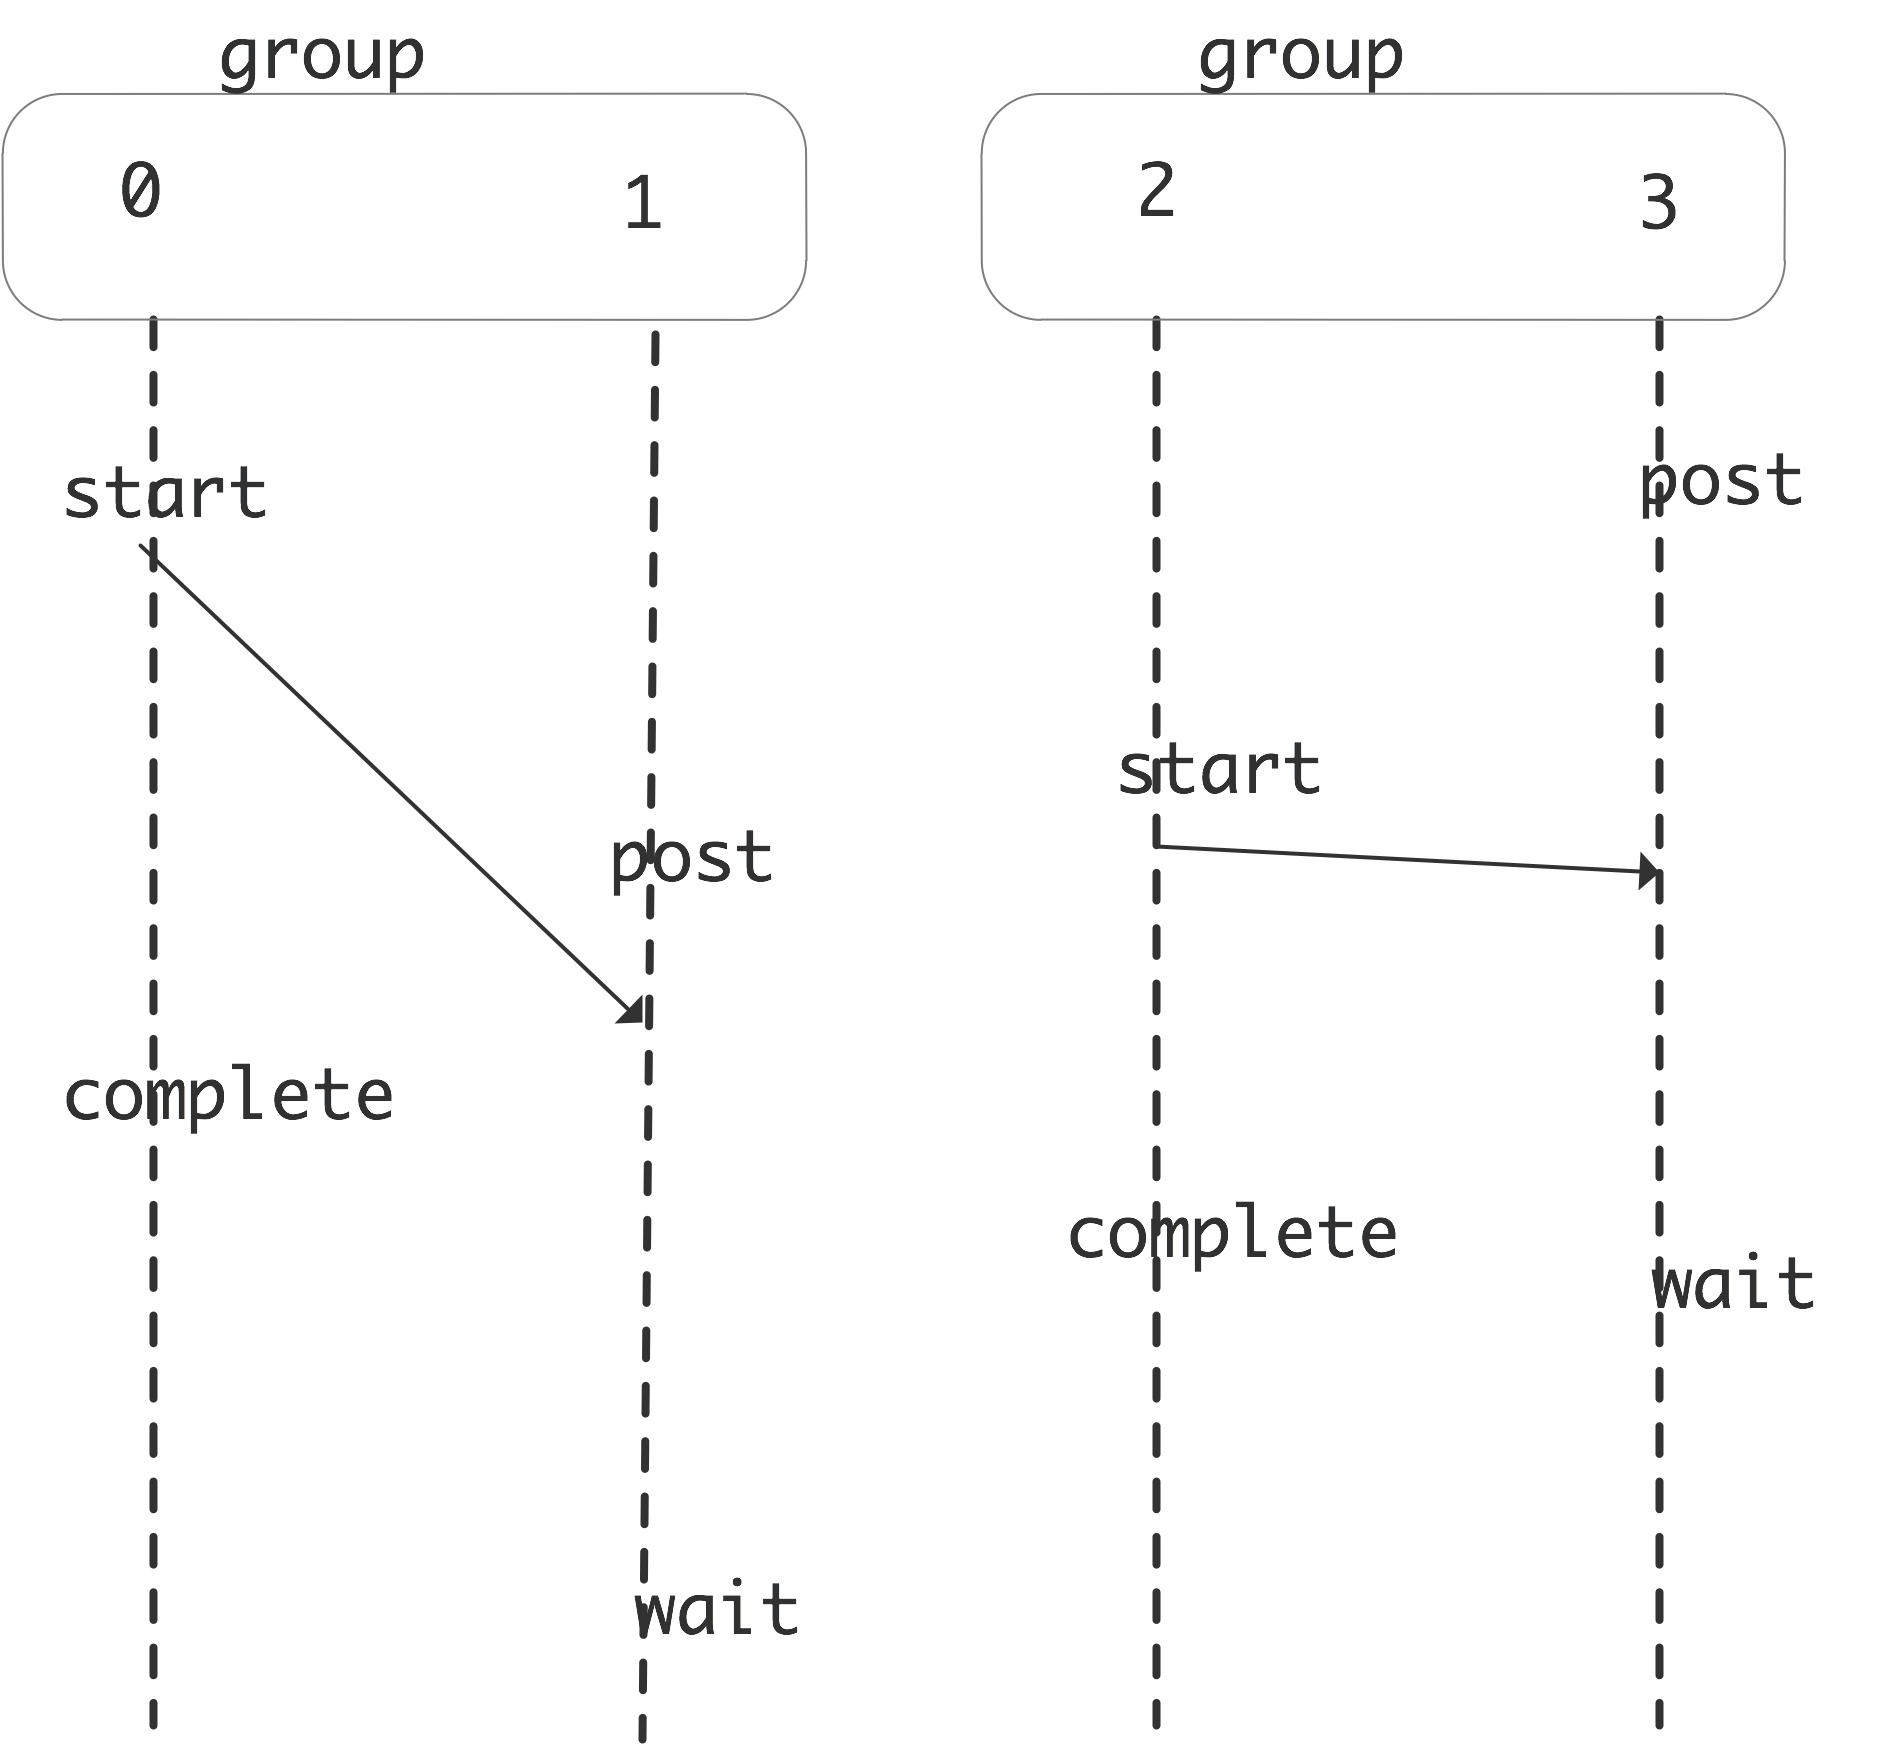
\includegraphics[scale=.1]{postwait}
  \caption{Window locking calls in fine-grained active target synchronization}
  \label{fig:postwait}
\end{figure}

You start and complete an \indextermsub{exposure}{epoch} with%
\indexmpi{MPI_Win_post}\indexmpi{MPI_Win_wait}:
\begin{verbatim}
int MPI_Win_post(MPI_Group group, int assert, MPI_Win win)
int MPI_Win_wait(MPI_Win win)
\end{verbatim}
In other words, this turns your window into the \indexterm{target} for a remote access.

You start and complete an \indextermsub{access}{epoch} with%
\indexmpi{MPI_Win_start}\indexmpi{MPI_Win_complete}:
\begin{verbatim}
int MPI_Win_start(MPI_Group group, int assert, MPI_Win win)
int MPI_Win_complete(MPI_Win win)
\end{verbatim}
In other words, these calls border the access to a remote window, with the current processor
being the \indexterm{origin} of the remote access.

In the following snippet a single processor puts data on one
other. Note that they both have their own definition of the group, and
that the receiving process only does the post and wait calls.
\verbatimsnippet{postwaittwo}

\Level 1 {Passive target synchronization}
\commandreflabel{passive-sync}

\indexmpi{MPI_Win_lock}\indexmpi{MPI_Win_unlock}
\begin{verbatim}
MPI_Win_lock (int locktype, int rank, int assert, MPI_Win win)
MPI_Win_unlock (int rank, MPI_Win win)
\end{verbatim}

The \indexmpi{MPI_Fetch_and_op} call atomically retrieves an item from the window
indicated, and replaces the item on the target by doing an accumulate on it
with the data on the origin.
\begin{verbatim}
int MPI_Fetch_and_op(const void *origin_addr, void *result_addr,
        MPI_Datatype datatype, int target_rank, MPI_Aint target_disp,
        MPI_Op op, MPI_Win win)
\end{verbatim}
\verbatimsnippet{fetchop}

\Level 0 {Collectives}

\Level 1 {Rooted collectives}
\commandreflabel{bcast}

The \indexmpishow{MPI_Bcast} call has a single data argument. Its
value on the root processor is copied to all other processors,
where any previous value is overwritten.
\begin{verbatim}
int MPI_Bcast( void *buffer, int count, MPI_Datatype datatype, int root, 
               MPI_Comm comm )
\end{verbatim}
There is an example in section~\ref{ref:mpi-init}.

The \indexmpishow{MPI_Reduce} call combines the values from the individual
processors. In order not to overwrite the input value on the root, 
this call has two data arguments, a send buffer and a receive buffer.
\begin{verbatim}
int MPI_Reduce
  (void *sendbuf, void *recvbuf, int count, MPI_Datatype datatype, 
   MPI_Op op, int root, MPI_Comm comm)
\end{verbatim}
On processes that are not the root, the receive buffer is ignored. 
\verbatimsnippet{reduce}

On the root, 
you need two buffers, which could be a significant memory demand
in the case of a large array to be reduced.
Therefore, you can specify \indexmpishow{MPI_IN_PLACE} as the send
buffer on the root. The reduction call then
uses the value in the receive buffer as the root's contribution to the operation.
\verbatimsnippet{reduceinplace}

In Fortran the code is less elegant because you can not do
these address calculations:
\verbatimsnippet{reduceinplace-f}

\Level 1 {Gather and scatter}
\commandreflabel{gatherscatter}

In the gather and scatter calls, each processor has $n$ elements of individual
data. There is also a root processor that has an array of length~$np$, where $p$
is the number of processors. The gather call collects all this data from the 
processors to the root; the scatter call assumes that the information is 
initially on the root and it is spread to the individual processors.

The prototype for \indexmpishow{MPI_Gather} has two `count' parameters, one
for the length of the individual send buffers, and one for the receive buffer.
However, confusingly, the second parameter (which is only relevant on the root)
does not indicate the total amount of information coming in, but
rather the size of \emph{each} contribution. Thus, the two count parameters
will usually be the same (at least on the root); they can differ if you 
use different \indexmpishow{MPI_Datatype} values for the sending and receiving
processors.
\begin{verbatim}
int MPI_Gather(
  void *sendbuf, int sendcnt, MPI_Datatype sendtype,
  void *recvbuf, int recvcnt, MPI_Datatype recvtype,
  int root, MPI_Comm comm
);
\end{verbatim}

Here is a small example:
\verbatimsnippet{gather}
This will also be the basis of a more elaborate example in
section~\ref{ref:v-collective}.

The \n{MPI_IN_PLACE} option can be used for the send buffer on the root;
the data for the root is then assumed to be already in the correct location
in the receive buffer.

The \indexmpishow{MPI_Scatter} operation is in some sense the inverse of the gather:
the root process has an array of length $np$ where $p$~is the number of processors
and $n$~the number of elements each processor will receive.
\begin{verbatim}
int MPI_Scatter
  (void* sendbuf, int sendcount, MPI_Datatype sendtype, 
   void* recvbuf, int recvcount, MPI_Datatype recvtype, 
   int root, MPI_Comm comm) 
\end{verbatim}

\Level 1 {Reduce-scatter}
\commandreflabel{reducescatter}

The \indexmpishow{MPI_Reduce_scatter} command is equivalent to a reduction
on an array of data, followed by a scatter of that data to the individual processes.

To be precise, there is an array \n{recvcounts} where \n{recvcounts[i]} gives
the number of elements that ultimate wind up on process~\n{i}.
The result is equivalent to doing a reduction with a length equal to the sum
of the \n{recvcounts[i]} values, followed by a scatter where process~\n{i}
receives \n{recvcounts[i]} values. (Since the amount of data to be scattered
depends on the process, this is in fact equivalent to \indexmpishow{MPI_Scatterv}
rather than a regular scatter.)
\begin{verbatim}
int MPI_Reduce_scatter
  (void* sendbuf, void* recvbuf, int *recvcounts, MPI_Datatype datatype, 
   MPI_Op op, MPI_Comm comm)
\end{verbatim}
For instance, if all \n{recvcounts[i]} values are~1, the sendbuffer has one element
for each process, and the receive buffer has length~1.

An important application of this is establishing an irregular
communication pattern.  Assume that each process knows which
other processes it wants to communicate with; the problem is to
let the other processes know about this.
The solution is to use \n{MPI_Reduce_scatter} to find out how many processes
want to communicate with you, and then wait for precisely that many messages
with a source value of \indexmpishow{MPI_ANY_SOURCE}.
\verbatimsnippet{reducescatter}

\Level 1 {`All'-type collectives}
\commandreflabel{allreduce}

The following collectives construct a result on all processes:
\indexmpishow{MPI_Allgather}
\begin{verbatim}
int MPI_Allgather
  (void *sendbuf, int sendcount, MPI_Datatype sendtype, 
   void *recvbuf, int recvcount, MPI_Datatype recvtype, 
  MPI_Comm comm)
\end{verbatim}
%
\indexmpishow{MPI_Allreduce}
\begin{verbatim}
int MPI_Allreduce 
  (void *sendbuf, void *recvbuf, int count, 
   MPI_Datatype datatype, MPI_Op op, 
   MPI_Comm comm )
\end{verbatim}
%
\indexmpishow{MPI_Alltoall}
\begin{verbatim}
int MPI_Alltoall
  (void *sendbuf, int sendcount, MPI_Datatype sendtype, 
   void *recvbuf, int recvcount, MPI_Datatype recvtype, 
   MPI_Comm comm)
\end{verbatim}
Each processor has a contribution in their send buffer; the global result
is returned in each processor's receive buffer.
\verbatimsnippet{allreduce}

If a large amount of data is being communicated, it may be wasteful to 
have both a (large) send and receive buffer.
This problem can be circumvented by using \indexmpishow{MPI_IN_PLACE}
as the specification of the send buffer. The send data is then
assumed to be in the receive buffer. After the reduction it is, of course,
overwritten.
\verbatimsnippet{allreduceinplace}

\Level 1 {Variable-size-input collectives}
\commandreflabel{v-collective}

There are various calls where processors can have
buffers of differing sizes.
\begin{itemize}
\item In \indexmpishow{MPI_Scatterv} the root process has a different
  amount of data for each recipient.
\item In \indexmpishow{MPI_Gatherv}, conversely, each process
  contributes a different sized send buffer to the received result;
  \indexmpishow{MPI_Allgatherv} does the same, but leaves its result
  on all processes; \indexmpishow{MPI_Alltoallv} does a different
  variable-sized gather on each process.
\end{itemize}

\begin{verbatim}
int MPI_Scatterv
  (void* sendbuf, int *sendcounts, int *displs, MPI_Datatype sendtype, 
   void* recvbuf, int recvcount, MPI_Datatype recvtype, 
   int root, MPI_Comm comm)
\end{verbatim}

\begin{verbatim}
int MPI_Gatherv
  (void *sendbuf, int sendcnt, MPI_Datatype sendtype,
   void *recvbuf, int *recvcnts, int *displs, MPI_Datatype recvtype,
   int root, MPI_Comm comm)
\end{verbatim}

\begin{verbatim}
int MPI_Allgatherv
  (void *sendbuf, int sendcount, MPI_Datatype sendtype, 
   void *recvbuf, int *recvcounts, int *displs, 
   MPI_Datatype recvtype, MPI_Comm comm)
\end{verbatim}

\indexmpishow{MPI_Alltoallv}.
\begin{verbatim}
int MPI_Alltoallv
  (void *sendbuf, int *sendcnts, int *sdispls, MPI_Datatype sendtype, 
   void *recvbuf, int *recvcnts, int *rdispls, MPI_Datatype recvtype,
   MPI_Comm comm)
\end{verbatim}

For example, in an \indexmpishow{MPI_Gatherv} call each process has an individual
number of items to contribute. To gather this, the root process needs
to find these individual amounts with an \n{MPI_Gather} call, and
locally construct the offsets array. Note how the offsets array has
size \n{ntids+1}: the final offset value is automatically the total
size of all incoming data.  
%
\verbatimsnippet{gatherv}

\Level 1 {Scan}
\commandreflabel{scan}

The scan operations are\indexmpi{MPI_Scan}
\begin{verbatim}
int MPI_Scan(void* sendbuf, void* recvbuf, 
    int count, MPI_Datatype datatype, MPI_Op op, MPI_Comm comm ) 
\end{verbatim}
and\indexmpi{MPI_Exscan}
\begin{verbatim}
int MPI_Exscan(void* sendbuf, void* recvbuf, 
    int count, MPI_Datatype datatype, MPI_Op op, MPI_Comm comm ) 
\end{verbatim}
The \n{MPI_Op} operations do not return an error code.

The result of the exclusive scan is undefined on processor~0,
and on processor~1 it is a copy of the send value of processor~1.
In particular, the \n{MPI_Op} need not be called on these two 
processors.

Scan operations are often useful in index calculations. Suppose that every processor
has part of a long array, and it knows only how many element it has. The following bit
computes the global index of its first element.\indexmpi{MPI_Exscan}
\verbatimsnippet{myfirst}

\Level 1 {Non-blocking collectives}
\commandreflabel{mpi3collect}

The same calling sequence as the blocking counterpart, except for the addition
of an \indexmpishow{MPI_Request} parameter. For instance 
\indexmpishow{MPI_Ibcast}:
\begin{verbatim}
int MPI_Ibcast(
  void *buffer, int count, MPI_Datatype datatype,
  int root, MPI_Comm comm, 
  MPI_Request *request)
\end{verbatim}

\Level 0 {Cancelling messages}

In section~\ref{sec:mpi-source} we showed a master-worker example where the 
master accepts in arbitrary order the messages from the workers.
Here we will show a slightly
more complicated example, where only the result of the first task to
complete is needed. Thus, we issue an \n{MPI_Recv}
with \indexmpishow{MPI_ANY_SOURCE} as source.  When a result comes, we
broadcast its source to all processes.  All the other workers then use
this information to cancel their message with
an \indexmpishow{MPI_Cancel} operation.

\verbatimsnippet{cancel}

\Level 0 {Communicators}

\Level 1 {Communicator duplication}
\commandreflabel{comm-dup}

In section~\ref{sec:mpi-semantics} it was explained that MPI messages are 
non-overtaking. This may lead to confusing situations, witness the following snippet:

\verbatimsnippet{wrongcatchmain}

This models a main program that does a simple message exchange, and it
makes two calls to library routines. Unbeknown to the user, the library also issues send and receive calls, and they turn out to interfere:

\verbatimsnippet{wrongcatchlib}

Here
\begin{itemize}
\item The main program does a send,
\item the library call \n{function_start} does a send and a receive;
  because the receive can match either send, it is paired with the
  first one;
\item the main program does a receive, which will be paired with the send of the 
  library call;
\item both the main program and the library do a wait call, and in
  both cases all requests are succesfully fulfilled, just not the way
  you intended.
\end{itemize}

The solution is to give the library a separate communicator with
\indexmpishow{MPI_Comm_dup}. Newly created communicators should be
released again with \indexmpishow{MPI_Comm_free}.

\verbatimsnippet{rightcatchmain}

\Level 1 {Splitting communicators}
\commandreflabel{comm-split}

The command \indexmpishow{MPI_Comm_split} takes a communicator, and
divides it into a number of disjoint communicators. It does this by
assigning processes to the same subcommunicator if they have the same
user-specified `colour' value.
\begin{verbatim}
int MPI_Comm_split(MPI_Comm comm, int color, int key, 
                   MPI_Comm *newcomm)
\end{verbatim}
The ranking of processes in the new communicator is determined by a `key' value.
Most of the time, there is no reason to use a relative ranking that is different from
the global ranking, so the \n{MPI_Comm_rank} value of the global communicator
is a good choice.
\verbatimsnippet{commsplitrowcol}

\Level 1 {Process topologies}
\commandreflabel{topology}

\Level 2 {Cartesian grid topology}
\commandreflabel{cartesian}

The cartesian topology is specified by giving
\indexmpishow{MPI_Cart_create} the sizes of the processor grid along
each axis, and whether the grid is periodic along that axis.
\begin{verbatim}
int MPI_Cart_create(
  MPI_Comm comm_old, int ndims, int *dims, int *periods, 
  int reorder, MPI_Comm *comm_cart)
\end{verbatim}
Each point in this new communicator has a coordinate and a rank.  They
can be queried with \indexmpishow{MPI_Cart_coord} and
\indexmpishow{MPI_Cart_rank} respectively.
\begin{verbatim}
int MPI_Cart_coords(
  MPI_Comm comm, int rank, int maxdims,
  int *coords);
int MPI_Cart_rank(
  MPI_Comm comm, init *coords, 
  int *rank);
\end{verbatim}
Note that these routines can give the coordinates for any rank,
not just for the current process.
%
\verbatimsnippet{cart}

The \n{reorder} parameter to \n{MPI_Cart_create}
indicates whether processes can have a rank
in the new communicator that is different from in the old one.

Strangely enough you can only shift in one direction, you can not
specify a shift vector.
\begin{verbatim}
int MPI_Cart_shift(MPI_Comm comm, int direction, int displ, int *source, 
                  int *dest)
\end{verbatim}
If you specify a processor outside the grid
the result is \indexmpishow{MPI_PROC_NULL}.

\Level 0 {Leftover topics}

\Level 1 {32-bit size issues}

The \n{size} parameter in MPI routines is defined as an \n{int},
meaning that it is limited to 32-bit quantities.  There are ways
around this, such as sending a number of
\indexmpishow{MPI_Type_contiguous} blocks that add up to more than~$2^{31}$.

\Level 1 {Fortran issues}
\commandreflabel{mpi-fortran}
\index{MPI!Fortran issues|(}

\Level 2 {Data types}

The equivalent of \indexmpishowsub{MPI_Aint}{in Fortran} is
\begin{verbatim}
integer(kind=MPI_ADDRESS_KIND) :: winsize
\end{verbatim}

\Level 2 {Type issues}

Fortran90 is a strongly typed language, so it is not possible to pass
argument by reference to their address, as C/C++ do with the \n{void*}
type for send and receive buffers. In Fortran this is solved by having
separate routines for each datatype, and providing an \n{Interface} block
in the MPI module. If you manage to request a version that does not exist,
the compiler will display a message like
\begin{verbatim}
There is no matching specific 
subroutine for this generic subroutine call [MPI_Send]
\end{verbatim}

\Level 2 {Byte calculations}
\label{sec:f-sizeof}

Fortran lacks a \n{sizeof} operator to query the sizes of datatypes.
Since sometimes exact byte counts are necessary,
for instance in one-sided communication,
Fortran can use the \indexmpishow{MPI_Sizeof} routine:
\begin{verbatim}
call MPI_Sizeof(windowdata,window_element_size,ierr)
window_size = window_element_size*500
call MPI_Win_create( windowdata,window_size,window_element_size,... );
\end{verbatim}

\index{MPI!Fortran issues|)}

\Level 0 {Error handling}
\commandreflabel{mpi:error}

MPI operators (\indexmpishow{MPI_Op}) do not return an error code. In case of
an error they call \n{MPI_Abort}; if \indexmpishow{MPI_ERRORS_RETURN}
is the error handler, errors may be silently ignore.

\Level 0 {More utility stuff}
\Level 1 {Timing}
\commandreflabel{timing}

MPI has a \indexterm{wall clock} timer: \indexmpishow{MPI_Wtime}
\begin{verbatim}
// C
double MPI_Wtime(void);
! F
DOUBLE PRECISION MPI_WTIME()
\end{verbatim}
which gives the number of seconds from a certain point in the past.
(Note the absence of the error parameter in the fortran call.)
\verbatimsnippet{pingpong}

The timer has a resolution of \indexmpishow{MPI_Wtick}:
\begin{verbatim}
double MPI_Wtick(void);
\end{verbatim}

Timing in parallel is a tricky issue. For instance, most clusters do
not have a central clock, so you can not relate start and stop times
on one process to those on another. You can test for a global clock as
follows\indexmpi{MPI_WTIME_IS_GLOBAL}:
\begin{verbatim}
int *v,flag;
MPI_Attr_get( comm, MPI_WTIME_IS_GLOBAL, &v, &flag );
if (mytid==0) printf(``Time synchronized? %d->%d\n'',flag,*v);
\end{verbatim}
%\indexmpi{MPI_Wtime} can be either a function or a macro.

%\Level 1 {Profiling}
%\commandreflabel{profile}

\Level 0 {Multi-threading}
\commandreflabel{mpi-thread}

\begin{verbatim}
int MPI_Init_thread( int *argc, char ***argv, int required, int *provided )
\end{verbatim}

\begin{itemize}
\item \indexmpishow{MPI_THREAD_SINGLE}: each MPI process can only have
  a single thread.
\item \indexmpishow{MPI_THREAD_FUNNELED}: an MPI process can be
  multithreaded, but all MPI calls need to be done from a single
  thread.
\item \indexmpishow{MPI_THREAD_SERIALIZED}: a processes can sustain
  multiple threads that make MPI calls, but these threads can not be
  simultaneous: they need to be for instance in an OpenMP
  \indexterm{critical section}.
\item \indexmpishow{MPI_THREAD_MULTIPLE}: processes can be fully
  generally multi-threaded.
\end{itemize}
